% Relatório referente ao projeto "Reconhecimento de Locutor Independente de
% Texto" entregue em 4 de Agosto de 2014, da disciplina "Processamento de Voz",
% ministrada pelo professor Tsang Ing Ren. O documento está no formato de paper
% do IEEE.

\documentclass[a4paper,twocolumn]{article}

\usepackage{times}
\usepackage[utf8]{inputenc}
\usepackage[english]{babel}
\usepackage[a4paper,margin=2cm,columnsep=1cm]{geometry}
\usepackage{authblk}
\usepackage{titlesec}
\usepackage[pdftex]{graphicx}
\usepackage{mathtools}


\begin{document}

\graphicspath{{images/}}
\renewcommand{\abstractname}{\normalsize\bfseries\filcenter ABSTRACT}
\titleformat*{\section}{\normalsize\bfseries\filcenter}
\titleformat*{\subsection}{\small\bfseries\filcenter}
\renewcommand{\refname}{\normalsize\bfseries\filcenter REFERENCES}
\renewcommand{\figurename}{\small Figure}
\newcommand{\figureref}[1]{\textit{Figure \ref{fig:#1}}}
\newcommand{\equationref}[1]{\textit{Equation \ref{eq:#1}}}
\newcommand{\bigsum}{\displaystyle\sum}


\title{\textbf{Speaker Verification Using Adapted Gaussian Mixture Models}}
\author{\textit{Sérgio R. F. Vieira, Eduardo M. B. de A. Tenório and Tsang Ing Ren}}
\affil{Centro de Informática, Universidade Federal de Pernambuco\\
Recife, PE, Brazil -- www.cin.ufpe.br\\
\small\texttt{\{srfv,embat,tir\}@cin.ufpe.br}}
\date{August, 2014}

\maketitle


\begin{abstract}
\begin{itshape}
Colocar o abstract aqui

\noindent\textbf{keywords}: colocar keywords aqui
\end{itshape}
\end{abstract}


\section{INTRODUCTION}
\label{intro}

Traditionally, strategies for verification and identification of a individual are based on some foreknowledge, like a password or a personal identification number. In other cases physical objects (like keys or cards) are used. The Achilles heel of theses strategies is the verification/identification object itself. Once a key is lost or a password is forgotten, the person cannot prove to be herself. In cases of theft, a malicious agent can easily impersonate the victim.

With the growing advancements in IT, biometric systems became more common and, in a self fed loop, more precise. The biometry of the voice is one of the most reliable and easy to use. To extract its features, the person just needs to speak, and if the system is well designed, it is very unlikely to an imposter be granted access. Many techniques based on statistical models exists, each one focused in a particular set of subproblems. Here we will use the Gaussian Mixture Models (GMM).

A GMM is a generic probabilistic model for multivariate densities capable of representing arbitrary densities, making it well suited for unconstrained text-independent applications. The use of GMMs for this type of speaker identification was first described in \cite{rose_reynolds_1990}, and since then, this approach has gained popularity and became the state of the art in text-independent speaker recognition applications. This fact is evidenced by numerous papers published in majors conferences, such as International Conference on Acoustics, Speech, and Signal Processing (ICASSP), the International Speech Communication Association (ISCA, formerly known as Eurospeech), and the International Conference on Spoken Language Processing (ICSLP), as well as articles in ESCA Transactions on Speech Communications and IEEE Transactions on Speech and Audio Processing.

This paper is a reduced reproduction of \cite{reynolds_quatieri_dunn_2000}, in which we present a Gaussian Mixture Model-Universal Background Model (GMM-UBM) and a GMM adapted from the GMM-UBM. These models are used to verify a speaker using the Likelihood-Ratio Test. The explanation is divided in the folowing sections: 2) \textit{Features Extraction}, in which the MFCC technique is briefly described; 3) \textit{GMM-UBM Training}, showing how to create a model to represent the utterances of all possible speakers; 4) \textit{Adaptation of Speaker Model}, showing how to use the GMM-UBM to derive a model for each speaker; 5) \textit{Likelihood-Ratio Test}, calculating a measure of how different a speaker is from the background; 6) \textit{Experiments} executed to validate the approach chosen; and 7) \textit{Conclusion}, in which the final considerations are given. The \textit{References} section at the end contains all the sources used to write the paper and conduct the experiments.

% TODO colocar na seção de experimentos
% The base used is MIT Mobile Device Speaker Verification Corpus, composed of three sessions of utterances: training (Enroll\_Session\_1), true speakers test (Enroll\_Session\_2) and imposters test (Imposter). The Enroll sessions contains 48 speakers and the Imposter session contains 40 speakers, with 59 utterances each. More details are given in \cite{corpus_paper}.


\section{FEATURES EXTRACTION}
\label{feat_ext}

The features extraction process transforms a speech signal into a vector containing the information needed to perform the verification/identification. In the case of text-independent verification, as shown in \cite{pinheiro_2013}, the features extracted must have: high variation inter-speakers and low variation intra-speakers; robustness in the presence of noise and distortion; be frequent and natural in speech; easy to measure and to extract from speech signal; hard to be artificially produced; be immutable, even in the presence of sickness or aging.

In this paper we used the Mel-Frequency Cepstral Coefficients (MFCCs) \cite{davis_mermelstein_1980} to perform the feature extraction, associated to their time derivatives and to the logarithm of the signal's energy. The Mel scale is derived from researches in human listening and is given by

\begin{equation}
    \label{eq:hertz_to_mel}
    mel = 2595\log_{10} (1 + \frac{f}{700})
\end{equation}

\noindent where \textit{f} is the frequency in Hertz. The log-scale improves the readability of lower frequencies, making it well suited for this kind of problem (the majority of human voice is under 4kHz).

\figureref{mfcc_flow} shows the MFCC extraction flow, receiving a representation of the physical signal and returning a vector of coefficients containing representing the almost unique characteristics of the speaker's voice.

\begin{description}
  \item[Pre-emphasis]
\end{description}

\begin{figure}[h]
    \label{fig:mfcc_flow}
    \centering
    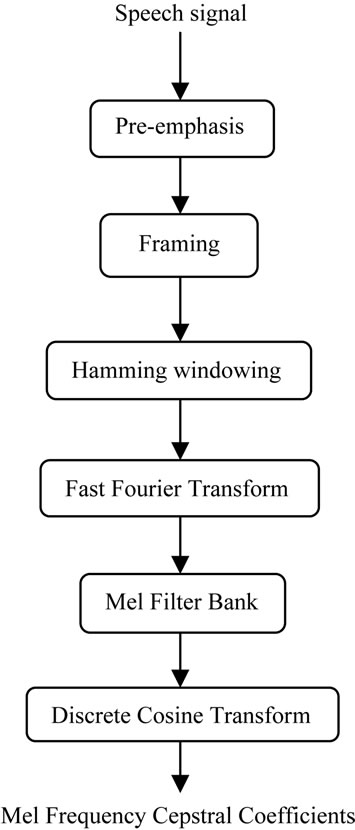
\includegraphics[scale=0.5]{mfcc-flow}
    \caption{\textit{Block diagram of MFCCs extraction from a speech signal.}}
\end{figure}


\begin{thebibliography}{9}
    \bibitem{rose_reynolds_1990}
        R. C. Rose and D. A. Reynolds,
        ``Text-independent speaker identification using automatic acoustic segmentation,"
        in \textit{Proc. of the International Conference on Acoustics, Speech, and
        Signal Processing},
        1990,
        pp. 293–296.

    \bibitem{reynolds_quatieri_dunn_2000}
        D. A. Reynolds et al.,
        ``Speaker verification using adapted gaussian mixture models,"
        \textit{Digital Signal Processing}, vol. 10,
        (1-3) pp. 19-41,
        2000.

    \bibitem{corpus_paper}
        R. H. Woo et al.,
        ``The MIT Mobile Device Speaker Verification Corpus: Data Collection and Preliminary Experiments,"
        in \textit{The Speaker and Language Recognition Workshop (IEEE Odyssey 2006),}
        San Juan, Puerto Rico, 2006.

    \bibitem{pinheiro_2013}
        H. N. B. Pinheiro,
        ``Sistemas de reconhecimento de locutor independente de texto,"
        B.Eng. monograph, Universidade Federal de Pernambuco,
        Recife, Pernambuco, Brazil,
        2013.

    \bibitem{davis_mermelstein_1980}
        S. B. Davis and P. Mermelstein,
        ``Comparison of Parametric Representations for Monosyllabic Word Recognition in Continuously Spoken Sentences,"
        in \textit{IEEE Trans. Acoust., Speech, Signal Process.},
        vol. 28
        pp. 357-366,
        Aug. 1980.

\end{thebibliography}

\end{document}